\chapter{Non-parametric approximation}
\section{Introduction}
The subject of the fourth laboratory class was non parametric approximation. 
The principle it is based on is orthogonal series expansion. Every function
can be approximated over some domain $\mathcal{D}$ by a series of orthogonal functions as follows:
\begin{equation}
    \label{serexp}
    f(x) = \Sigma_{i=0}^{\infty} a_i g_i(x)
\end{equation}
where $a_i$ are constant coefficients, and $g_i$ fulfill the following property:
\begin{equation}
    \label{ort}
    \int_{\mathcal{D}} g_i(x) g_j(x) dx = 0 \text{ for }i \neq j
\end{equation}
If the basis functions are not just orthogonal, but orthonormal, then we also have:
\begin{equation}
    \label{nor}
    \int_{\mathcal{D}} g_i^{2}(x)dx = 1
\end{equation}

The way to obtain the coefficient $a_j$ is to multiply the original equation \ref{serexp} by the basis function it is associated with, and integrate the both sides over the domain $\mathcal{D}$.
\begin{equation}
    \begin{aligned}
        f(x)&= \Sigma_{i=1}^{\infty}a_ig_i(x)&\mbox{Multiply both sides by some $g_j(x)$}\\[1.25ex]
        f(x)g_j(x)&= \Sigma_{i=1}^{\infty}a_ig_i(x)g_j(x)&\mbox{Integrate over $\mathcal{D}$}\\[1.25ex]
        \int_{\mathcal{D}}f(x)g_j(x)dx&= a_j&\mbox{By \ref{ort} and \ref{nor}, all other coefficients cancel out}$\\[1.25ex]
    \end{aligned}
\end{equation}
There are 2 problems with the above formula. The first is that it requires a priori knowledge of $f(x)$, and the second that it requires a continuum of measurements over the whole domain $\mathcal{D}$. To remedy both problems one can use the fact, that $a_j$ can be interpreted as an expected value:
\begin{equation}
        a_j = E[g_j(x)]
\end{equation}
Which means that it can be estimated as an arithmetic mean of a set of measurements as follows:
\begin{equation}
     \hat{a}_j = \frac{1}{N}\Sigma_{i=1}^{N}g_j(x_i)
\end{equation}
All this leads to the following conclusion: \\
Given a set of orthonormal functions, and a sequence of independent random variables $x = x_1,\cdots ,x_k,\cdots x_N$ we can approximate their distribution function using its orthonormal expansion without assuming anything about it -- thus making this method non-parametric. What's more we obtain a sequence of approximations parametrised by the number of terms of the original sequence which we wish to keep:
\begin{equation}
    \hat{f}_S(x) = \Sigma_{i=0}^{S} \hat{a}_i g_i(x)
\end{equation}

\clearpage
\section{Laboratory}

During the class we were divided into 2 groups, with each group being given a distribution to approximate:

\begin{figure}[h!]
\begin{center}
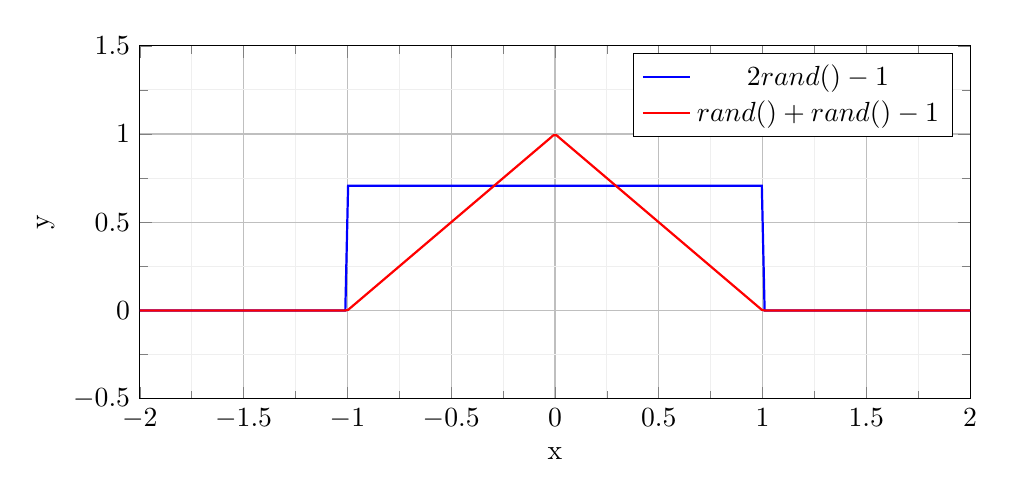
\begin{tikzpicture}
 
\begin{axis}[
    xmin = -2, xmax = 2,
    ymin = -0.5, ymax = 1.5,
    grid = both,
    minor tick num = 1,
    major grid style = {lightgray},
    minor grid style = {lightgray!25},
    width = \textwidth,
    height = 0.5\textwidth,
    xlabel = x,
    ylabel = y]
    \addplot[
        domain = -2:2,
        samples = 300,
        thick,
        blue,
        ] 
        {
        (x > -1)*(x < 1)*(1/sqrt(2))
        };


    \addplot[
        domain = -2:2,
        samples = 300,
        smooth,
        thick,
        red,
        ] 
        {
        (x < -1)*(0) +
        (x > -1)*(x < 0)*(1 + x) +
        (x > 0)*(x < 1)*( 1 - x) +
        (x > 1)*(0)
        };

    \legend{$2\text{rand}()-1$,
    $\text{rand}()+\text{rand}()-1$}
\end{axis}
 
\end{tikzpicture}
\end{center}
\caption{The group the author was is was given the triangle distribution}
\end{figure}

The goal was to use orthonormal series expansion to approximate either of those distributions, and see how the number of terms and number of samples affects the outcome of this approximation. 
\subsection{Approximation}
The chosen orthonormal basis was a set of trigonometric functions:
\begin{equation}
    g_i(x) = \begin{cases}
        \frac{1}{\sqrt{2}}\text{ if } i = 1\\
        \sin{(ix\frac{\pi}{2})} \text{ if } i > 1,\;  i \equiv 0 \mod{2}\\
        \cos{((i-1)x\frac{\pi}{2})} \text{ if } i > 1,\;  i \equiv 1 \mod{2}
    \end{cases}
\end{equation}

\begin{figure}[h!]
\begin{center}
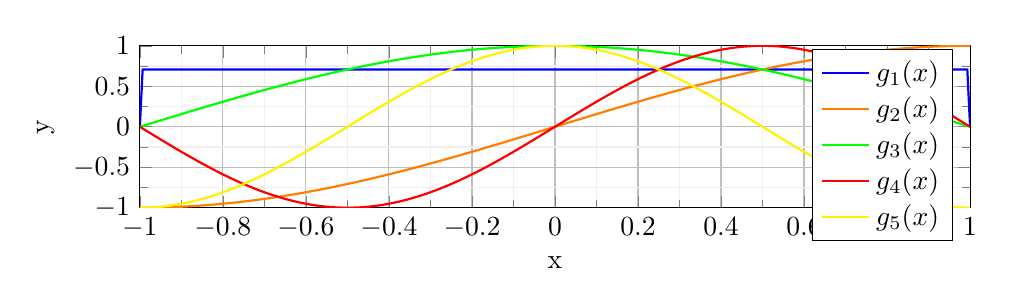
\begin{tikzpicture}
 
\begin{axis}[
    xmin = -1, xmax = 1,
    ymin = -1, ymax = 1,
    grid = both,
    minor tick num = 1,
    major grid style = {lightgray},
    minor grid style = {lightgray!25},
    width = \textwidth,
    height = 0.3\textwidth,
    xlabel = x,
    ylabel = y]
    \addplot[
        domain = -1:1,
        samples = 300,
        thick,
        blue,
        ] 
        {
        (x > -1)*(x < 1)*(1 / sqrt(2)) +0
        };

        \addplot[
        domain = -1:1,
        samples = 300,
        thick,
        orange,
        ] 
        {
        sin(deg(x)*3.1415/2)
        };

        \addplot[
        domain = -1:1,
        samples = 300,
        thick,
        green,
        ] 
        {
        (cos(deg(x)*3.1415/2)) +0
        };
        \addplot[
        domain = -1:1,
        samples = 300,
        thick,
        red,
        ] 
        {
       sin(deg(x)*3.1415)) + 0
        };
        \addplot[
        domain = -1:1,
        samples = 300,
        thick,
        yellow,
        ] 
        {
       (cos(deg(x)*3.1415)) + 0
        };




    \legend{
        $g_1(x)$,
        $g_2(x)$,
        $g_3(x)$,
        $g_4(x)$,
        $g_5(x)$}
\end{axis}
 
\end{tikzpicture}
\end{center}
\end{figure}



Armed with this basis, a script was written which would calculate all the necessary coefficients, as well as plot the resulting approximate distribution functions.
\clearpage
The resulting approximate distributions $\hat{f}_s(x)$ are shown below:
\begin{figure}[h!]
\begin{center}
\begin{tikzpicture}
 
\begin{axis}[
    xmin = -1, xmax = 1,
    ymin = 0, ymax = 1.25,
    grid = both,
    minor tick num = 1,
    major grid style = {lightgray},
    minor grid style = {lightgray!25},
    width = \textwidth,
    height = 0.5\textwidth,
    xlabel = x,
    ylabel = y]

    \addplot[color=blue,
        ]
        table [col sep=space, x index = 0, y index=1]{./plot_data/chapter_3/trig_app.dat};

    \addplot[color=yellow,
        ]
        table [col sep=space, x index = 0, y index=2]{./plot_data/chapter_3/trig_app.dat};

    \addplot[color=red,
        ]
        table [col sep=space, x index = 0, y index=3]{./plot_data/chapter_3/trig_app.dat};

    \addplot[color=green,
        ]
        table [col sep=space, x index = 0, y index=4]{./plot_data/chapter_3/trig_app.dat};

    \addplot[color=orange,
        ]
        table [col sep=space, x index = 0, y index=5]{./plot_data/chapter_3/trig_app.dat};

    \legend{
        $S = 1$,
        $S = 5$,
        $S = 10$,
        $S = 20$,
        $S = 50$}
\end{axis}
\end{tikzpicture}
\end{center}

\label{app_fig}
\caption{$\hat{f}_s(x)$ for $N = 10000$}
\end{figure}


From this, it is clear that simply increasing the number of terms of the approximation doesn't lead to better approximation. It's quiet evident, that at $S = 50$ the approximated distribution is more noisy than at $S = 20$. In fact, if we plot the error between the true distribution and its approximation as a function of the number of terms, we get the following plot:
%%

\begin{figure}[h!]
\begin{center}
\begin{tikzpicture}
 
\begin{axis}[
    xmin = 1, xmax = 1000,
    ymin = 0, ymax = 5,
    grid = both,
    minor tick num = 1,
    major grid style = {lightgray},
    minor grid style = {lightgray!25},
    width = 0.45\textwidth,
    height = 0.5\textwidth,
    xlabel = s,
    ylabel = $\norm{f(x)-\hat{f}_s(x)}^{2}_2$,
    scaled x ticks=false]


    \addplot[color=blue,
        ]
        table [col sep=space, x index = 0, y index=1]{./plot_data/chapter_3/trig_error.dat};

    %\legend{
    %    $\norm{f(x)-\hat{f}_s(x)}_2$,
%    $\hat{f}_1(x)$,
%    $\hat{f}_5(x)$,
%    $\hat{f}_{10}(x)$,
%$\hat{f}_{20}(x)$,
%$\hat{f}_{50}(x)$,
%}
\end{axis}
\end{tikzpicture}
\begin{tikzpicture}
\begin{axis}[
    xmin = 1, xmax = 100,
    ymin = 0, ymax = 5,
    grid = both,
    minor tick num = 1,
    major grid style = {lightgray},
    minor grid style = {lightgray!25},
    width = 0.45\textwidth,
    height = 0.5\textwidth,
    xlabel = s,
    ylabel = $\norm{f(x)-\hat{f}_s(x)}^{2}_2$,
    scaled x ticks=false]


    \addplot[color=blue,
        ]
        table [col sep=space, x index = 0, y index=1]{./plot_data/chapter_3/trig_error.dat};

    %\legend{
    %    $\norm{f(x)-\hat{f}_s(x)}_2$,
%    $\hat{f}_1(x)$,
%    $\hat{f}_5(x)$,
%    $\hat{f}_{10}(x)$,
%$\hat{f}_{20}(x)$,
%$\hat{f}_{50}(x)$,
%}
\end{axis}
\end{tikzpicture}
\caption{Square of the $L_2$ Norm of the error for a sequence of length $N = 10000$. Both plots show the same data over a different range.}
\end{center}
\end{figure}



At the beginning the error does decrease, but it starts growing linearly without bound after passing a certain minimum value. This suggests that for a given number of terms in the observed sequence, there is an optimal number of terms in the approximation. 
\clearpage
To investigate this relationship, 10 sequences of length N were generated. For each sequence the optimum number of terms is found, and finally their values are averaged. These averages were then plotted as a function of N.
\begin{equation}
    \hat{S}_{opt}(N) = \frac{1}{10}\Sigma_{i=1}^{10} \argmin_s{\norm{f(t) - \hat{f}_i(s,t,N)}^{2}_2}
\end{equation}
The following plots resulted for the triangular distribution:

\begin{figure}[h!]
\begin{center}
\begin{tikzpicture}
\begin{axis}[
    xmin = 1, xmax = 100000,
    ymin = 0, ymax = 20,
    grid = both,
    minor tick num = 1,
    major grid style = {lightgray},
    minor grid style = {lightgray!25},
    width = 0.45\textwidth,
    height = 0.5\textwidth,
    xlabel = N,
    ylabel = $\hat{S}_{opt}(N)$,
    scaled x ticks=false]

    \addplot[color=blue,
        ]
        table [col sep=space, x index = 0, y index=1]{./plot_data/chapter_3/opt_s.dat};

\end{axis}
\end{tikzpicture}
\begin{tikzpicture}
\begin{semilogxaxis}[
    xmin = 1, xmax = 100000,
    ymin = 0, ymax = 20,
    grid = both,
    minor tick num = 1,
    major grid style = {lightgray},
    minor grid style = {lightgray!25},
    width = 0.45\textwidth,
    height = 0.5\textwidth,
    xlabel = N,
    ylabel = $\hat{S}_{opt}(N)$,
    scaled x ticks=false]

    \addplot[color=blue,
        ]
        table [col sep=space, x index = 0, y index=1]{./plot_data/chapter_3/opt_s.dat};

\end{semilogxaxis}
\end{tikzpicture}

\caption{Plot of the optimal value of S as a function of N. The left plot uses a linear scale, while the right one uses a logarithmic scale for the arguments.}
\end{center}
\end{figure}

From the above figure we can conclude, that the optimal number of terms in the trigonometric orthonormal approximation of the triangle distribution grows logarithmically -- about 5 new terms per decade -- with the length of the sequence used for estimation. This result shows, that one can use just a few terms of the expansion to obtain satisfactory results, but the number of samples has to be fairly large. This can be seen in \ref{app_fig}, where even for 10000 samples the resulting approximations are still quite far from a triangle. It took a non-insignificant amount of time to obtain these plots, which would make extending this analysis to more distribution functions quite difficult. This is due to the fact that generating samples from these distributions can be by itself computationally intensive.

\section{Conclusions}
It is quiet remarkable how well non-parametric approximation works, especially given how universal it is. A comparatively large number of samples is required to closely approximate a given distribution function, but satisfactory results are obtained even for just a few terms. This number is likely larger for more complex distribution functions.
